\documentclass{article}

\usepackage{url,hyperref}
\usepackage{graphicx}
\usepackage{enumitem}
\usepackage{amsmath,amssymb,array,comment,eucal}
\usepackage[linesnumbered,ruled]{algorithm2e}
\usepackage{listings}
\usepackage{tikz}
\usetikzlibrary{automata,positioning}
\newcommand{\gap}{\vspace{6mm}}

\usepackage{Sweave}
\begin{document}
\Sconcordance{concordance:hw02_kk319_binary_search_tree_and_randomization.tex:hw02_kk319_binary_search_tree_and_randomization.Rnw:%
1 12 1 1 0 382 1}

\title{COMPSCI531 Fall19 Homework 2: Binary Search Trees and Randomization}
\author{Kuei-Yueh Ko}
\maketitle

%%%%% Outer Enumeration for All Questions %%%%%
\begin{enumerate}

%%%%%%%%%%%%%%%%%%%%%%%%%%%%%%%%%%%%%%%%%%%%%%%%%%%%%%%%%%%%%%%%%
%%% Q1 Binary Search Trees (BSTs)
%%%%%%%%%%%%%%%%%%%%%%%%%%%%%%%%%%%%%%%%%%%%%%%%%%%%%%%%%%%%%%%%%
\item  Binary Search Trees (BSTs)

%%%%% Inner Enumeration for Q1 %%%%%
\begin{enumerate}[label*=\arabic*.]

%%%%%%%%%%%%%%%%%%%%%%%%%%%%%%%%%%%%%%%%%%%%%%%
%%% Q1.1 
%%% Minimum greater value in binary search tree
%%%%%%%%%%%%%%%%%%%%%%%%%%%%%%%%%%%%%%%%%%%%%%%
\item Minimum greater value in binary search tree

Given a balanced binary search tree that has a total of n nodes, design an algorithm that finds the minimum value in the tree that is greater than a given value x, and justify the complexity of your algorithm. Your algorithm should run in O(logn) time for full credit
\gap

\textbf{My Answer}


Suppose we have a node connection as follow:

% Plot tree image with three nodes, labeled as A, B, C
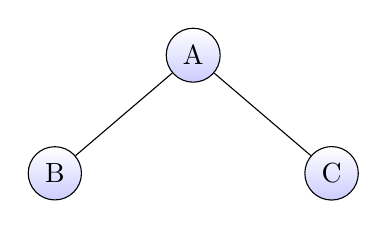
\begin{tikzpicture}[sibling distance=10em,
    % node attributes
    every node/.style = {
        shape=circle, 
        draw, 
        align=center,
        top color=white, 
        bottom color=blue!20}]]
    % layout tree structure  
    \node {A}
        child{ node{B} }
        child{ node{C} };
\end{tikzpicture}
% End of plotting tree

According to the definition of BST, the values of B and all its descendant are smaller than A, while the values of C and all its descendant are larger than A. As a results, there are four possible cases for an given input x:

\begin{itemize}
    \item 1. B < x < A < C
	  \item 2. B < A < x < C
	  \item 3. x < B
	  \item 4. C < x  
\end{itemize}

For case 1, A is our answer, because A is the smallest value comparing to C and its descendant. For case 2, we need to transverse to the right subtree (C and its descendant) to continue searching. If case 3 occur, we need to move to the left subtree to continue searching. For case 4, the we need to search at the right subtree.

Moreover, there are possibilities that we encounter the situation where the left or right subtree does not exit. To write down the algorithm above, we have

\begin{algorithm}[H]
\SetAlgoLined
\SetNoFillComment
    \caption{FindMinOfGreater(node, x)}
     
    \tcc{Initialization}
    rnode = node.right \\
    lnode = node.left  \\
    rval  = rnode.value\\
    lval  = lnode.value\\
    val   = node.value \\
    
    \tcc{Four possible cases}
    \Case{ lval < x < val < rval }{
        return val
    } 
    \Case{ lval < val < x < rval }{
        \uIf{ rnode $\neq$ NULL }{
            result = FindMinOfGreater(rnode, x)
        } \Else {
            result = FindMinOfGreater(lnode, x)
        } 
        
        \uIf{ result = NULL }{
            return rval
        } \Else {
            return result
        }
    }
    \Case{ rval < x } {
        \uIf{ lnode $\neq$ NULL }{
            result = FindMinOfGreater(lnode, x)
        } \Else {
            result = FindMinOfGreater(rnode, x)
        } 
        
        \uIf{ result = NULL }{
            return NULL
        } \Else {
            return result
        }
    }
    \Case{ lval < x } {
        return NULL
    }
\caption{How to write algorithms}
\end{algorithm}
\gap

Since what this search does is merely searching down the tree, the time complexity of the algorithm is the same as the height of the tree. That is, the algorithm should run in $O(logn)$.


\gap
%%%%%%%%%%%%%%%%%%%%%
%%% Q1.2 Radix Tree
%%%%%%%%%%%%%%%%%%%%%
\item Radix Tree

For a set of distinct strings $S$ whose lengths sum to n, lexicographically sort the string set S in $\Theta(n)$ time.
\gap

\textbf{My Answer}

The goal here is to construct a radix tree that represent the collection of all strings in a given set.

Suppose we have only four letters ATCG for each alphabet, we can construct a node with array of pointers where each pointer representing a specific letter. (The letters can be extended to all 26 alphabets as well; here I am just assuming there are four possible letters.) Here I will demonstrate the idea using python, and the array of pointers is illustrated using a dictionary of references.

\begin{lstlisting}[language=Python]
class Node():
    def __init__(self):
        dct = dict()
        dct["A"] = None
        dct["T"] = None
        dct["C"] = None
        dct["G"] = None
        self.dct = dct
        
    def add_child(self, base):
        new_node = Node()
        self.dct[base] = new_node
        return new_node
    
    def get_child(self, base):
        return self.dct[base]
    
    def is_null(self, base):
        return self.dct[base] == None 
    
    def is_leaf(self):
        for base in "ATCG":
            if not self.is_null(base):
                return False
        return True
\end{lstlisting}

Using this type of node, we could construct a tree for all the given strings. For each string, a child is added if a letter appears. For example, if the first letter is A, then the algorithm will have first pointer of the root node pointed to an empty node. That is, we add a child under the pointer A. For each given string, the tree constructing process will iterate through the letters and continue to grow the tree by adding nodes. Below is how I implemented the idea:

\begin{lstlisting}[language=Python]
def build_tree(root, string):
    cur = root
    for base in string:
        if cur.is_null(base):
            cur = cur.add_child(base)
        else:
            cur = cur.get_child(base)
\end{lstlisting}

Given an example of three strings, where string1 < string3 < string2

\begin{lstlisting}[language=Python]
root = Node()
string1 = "ATACG"
string2 = "ATGCC"
string3 = "ATACC"

build_tree(root, string1)
build_tree(root, string2)
build_tree(root, string3)
\end{lstlisting}

We have the tree structure as follow:
\begin{lstlisting}
A
-T
--A
---C
----C
----G
--G
---C
----C
\end{lstlisting}

The lexically sorted string can be acquired by how we recursively iterating the possible letters. For example, let's assuming A > C > G > T. When transversing through the tree, each string is collected/printed as a leaf is encountered.

\begin{lstlisting}
def get_string(node, string=""):
    for base in "ACGT":
        if not node.is_null(base):
            node_next = node.get_child(base)
            get_string(node_next, string + base)
    if node.is_leaf():
        print(string)
\end{lstlisting}

We then could print a lexically sorted strings, even though they are not input in order during the tree building part.

\begin{lstlisting}
>>> get_string(cur)
ATACC
ATACG
ATGCC
\end{lstlisting}

Suppose we iterate the nodes by assuming G > A > C > T, we will get different order of strings

\begin{lstlisting}
def get_string(node, string=""):
    for base in "GACT":
        if not node.is_null(base):
            node_next = node.get_child(base)
            get_string(node_next, string + base)
    if node.is_leaf():
        print(string)
\end{lstlisting}

\begin{lstlisting}
>>> get_string(cur)
ATGCC
ATACG
ATACC
\end{lstlisting}

To get the time complexity of the radix tree sorting, since we only iterate all the letters once during the tree building and iterate all the nodes once when output sorted strings, the time complexity for the string sorting algorithm using radix tree is therefore $\Theta(n)$

\gap
\end{enumerate}
%%%%% End Inner Enumeration for Q1 %%%%%

%%%%%%%%%%%%%%%%%%%%%%%%%%%%%%%%%%%%%%%%%%%%%%%
%%% Q2
%%% Randomized algorithms
%%%%%%%%%%%%%%%%%%%%%%%%%%%%%%%%%%%%%%%%%%%%%%%
\item  Randomized algorithms: design and analysis

%%%%% Inner Enumeration for Q2 %%%%%
\begin{enumerate}[label*=\arabic*.]

%%%%%%%%%%%%%%%%%%%%%
%%% Q2.1 Uneven coin flips
%%%%%%%%%%%%%%%%%%%%%
\item Uneven coin flips
\gap


\textbf{My Answer}

Since we know the probability of HT and TH are the same, one procedure is to set up two events based on HT and TH outcome, respectively. Based on this idea, we could have the process below:

% Plot tree image for markov chain illustration
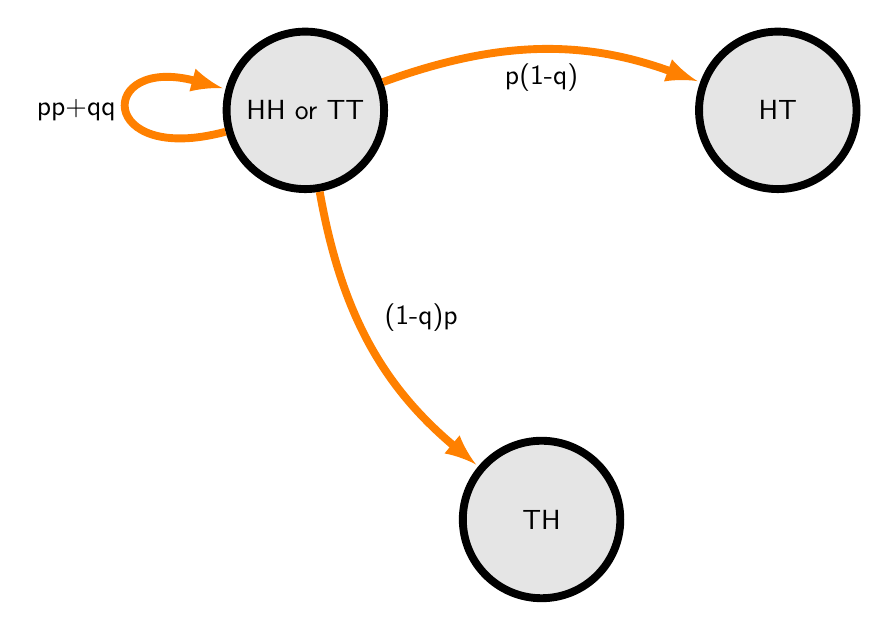
\begin{tikzpicture}[font=\sffamily]
    % Setup the style for the states
    \tikzset{node style/.style={
        state, 
        minimum width=2cm,
        line width=1mm,
        fill=gray!20!white}}
    % Draw the states
    \node[node style] at (0, 0)      (HHTT) {HH or TT};
    \node[node style] at (6, 0)      (HT)   {HT};
    \node[node style] at (3, -5.196) (TH)   {TH};

    % Connect the states with arrows
    \draw[every loop,
          auto=right,
          line width=1mm,
          >=latex,
          draw=orange,
          fill=orange]
        (HHTT) edge[bend left=20,  auto=right] node {p(1-q)} (HT)
        (HHTT) edge[bend right=20, auto=left]  node {(1-q)p} (TH)
        (HHTT) edge[loop left]                 node {pp+qq}  (HHTT);
\end{tikzpicture}
% End Plot tree image

The unbiased outcome Z can therefore be setup as

$$ Z = 
\begin{cases}
1 & \text{if we get a first HT for double coin toss} \\
0 & \text{if we get a first TH for double coin toss}
\end{cases}
$$

$Pr(Z = 1) = Pr(Z = 0) = \frac{1}{2}$ since the probability of getting HT and TH is symmetric.

Each sequence of double coin toss ends until the state $HT$ or the state $TH$ appear. The number of double coin toss can therefore be modeled by geometric distribution.

$$X = \text{\#double coin toss} \sim \text{Geo}(2p(1-q))$$

The geometric distribution here is the number of failure + one success. Thus, the p.m.f of $X$ is 
$$Pr(X) = (pp+qq)^{k-1}(2p(1-q))$$

The expected number of $X$, which is the expected number of trials for each time we draw a value from $Z$, is $\frac{1}{Pr(\text{getting HT or TH})} = \frac{1}{2p(1-q)}$

\gap
%%%%%%%%%%%%%%%%%%%%%
%%% Q2.2 Finding seats
%%%%%%%%%%%%%%%%%%%%%
\item Finding seats
Given n epople and m seats here m $leq$ n. People find seats by the following scheme:

%%% End Inner Enumeration for Q2.2 %%%
\begin{enumerate}[label=(\roman*)]
\item People find seats in a pre-determined order, i.e. no two or more people will try to find a seat at the same time
\item Every person will randomly choose one out of the m seats at uniform probability. If he/she finds that the seat is occupied by other person, he/she will repeat the random choosing scheme once again out of the m seats, until he/she finds a seat, or he/she has failed k times in total (k is a pre-determined positive integer).
\item A person will report to the administrator once he/she has failed k times, and the administrator will randomly assign an unoccupied seat for him/her.
\end{enumerate}
%%% End Inner Enumeration for Q2.2 %%%
Find the expected value of the number of people that have reported to the administrator at the end of this procedure. The answer should be a function of m, n and k and should be simplified at your best effort (thight asymptotic bounds suffice).
\gap

\textbf{My Answer}

The succeed rate and failure rate for each person enter is:

$$
\begin{cases}
p_i = 1 - \frac{i-1}{m} \\
q_i = \frac{i-1}{m}
\end{cases}
\text{for $i$ from 1 to $n$}
$$

The number of trails each person needs to take to find a seat (without the help from administrator) can be modeled by geometric distribution

$$X \sim Geo(p_i)$$

The p.m.f of X is

$$Pr(X=k) = (1-p_i)^{k-1}(p_i)$$

The cumulative distribution of X is

$$F(X=k) = Pr(X \leq k) = 1 - (1-p_i)^k$$

A person report to the administrator once he/she has failed k times; that is, the total trials he/she has is (k+1). Let the variate $Z_i$ be an indicator random variable of the trails. $Z_i$ is one if the $i^{th}$ person report to the administrator and zero otherwise.

$$Z_i = 
\begin{cases}
0 & \text{if failure $< k$ = total trials $< (k+1)$ = total trials $\leq k = X_i \leq k$} \\
1 & \text{otherwise}

\end{cases}
$$

$$Pr(Z_i) = 
\begin{cases}
Pr(Z_i = 0) = Pr(X_i \leq k)  & = 1 - (1-p_i)^{k} \\
Pr(Z_i = 1) = 1 - Pr(Z_i = 0) & = (1-p_i)^{k} 
\end{cases}
$$

The expected of total number of people reported can be calcualted as follow:

\begin{align*}
E[\sum_1^n Z_i] 
    = & \sum_{i=1}^n E[Z_i] \\
    = & \sum_{i=1}^n Pr(Z_i) \\
    = & \sum_{i=1}^n (1-p_i)^{k} \\
    = & \sum_{i=1}^n (\frac{i-1}{m})^{k} \\
    = & m^{-k} \sum_{i=1}^n (i-1)^{k} \\
    = & m^{-k} (0 + 1^k + 2^k + \dots + (n-1)^k) \\
    = & m^{-k} (n^k + O(n^{k-1}) \\
    = & ( \frac{n}{m} )^k + m^{-k} O\big( n^{k-1} \big)
\end{align*}

\gap
\end{enumerate}
%%%%% End Inner Enumeration for Q2 %%%%%

\end{enumerate}
\end{document}
